\section{ARQUITETURA DA INFRAESTRUTURA}

\subsection{Topologia Física e Lógica}

A infraestrutura do Cenário 03 é constituída por 20 dispositivos e 14 enlaces físicos comutados e dedicados, conforme ilustrado na Figura~\ref{fig:topologia_real}:
\begin{itemize}[leftmargin=2em]
  \item \textbf{Camada de Roteamento:} 1 roteador Cisco 1941 (\texttt{Router\_TI\_CBCC\_2026}), responsável pelo isolamento e encaminhamento entre os domínios de difusão das sub-redes departamentais e pela hospedagem dos serviços centrais de rede.
  \item \textbf{Camada de Comutação:} 2 comutadores gerenciáveis Cisco Catalyst 2960-24TT (\texttt{Switch\_01} e \texttt{Switch\_02}), fornecendo conectividade \textit{FastEthernet} e agregação de portas para as estações de trabalho e equipamentos sem fio.
  \item \textbf{Servidores e Estações Finais (Hosts):} 1 servidor central corporativo (\texttt{Server0}) com IP estático, 4 estações cabeadas (\texttt{PC0} a \texttt{PC3}), 4 computadores portáteis (\texttt{Laptop0} a \texttt{Laptop3}), 1 impressora de rede (\texttt{Printer0}) e dispositivos móveis adicionais.
  \item \textbf{Controladoras e Pontos de Acesso Sem Fio:} 2 controladoras \textit{Wireless LAN Controller} (\texttt{WLC-PT}) interligadas por cabos cruzados e 2 pontos de acesso leves \textit{Lightweight Access Point} (\texttt{LAP-PT}) provendo cobertura Wi-Fi para os dois setores.
  \item \textbf{Terminais de Console (Gerência Out-of-Band):} 3 enlaces dedicados com cabo de rollover (\texttt{eRollOver}) conectando estações portáteis diretamente às portas de console dos comutadores e do roteador.
\end{itemize}

\begin{figure}[H]
    \centering
    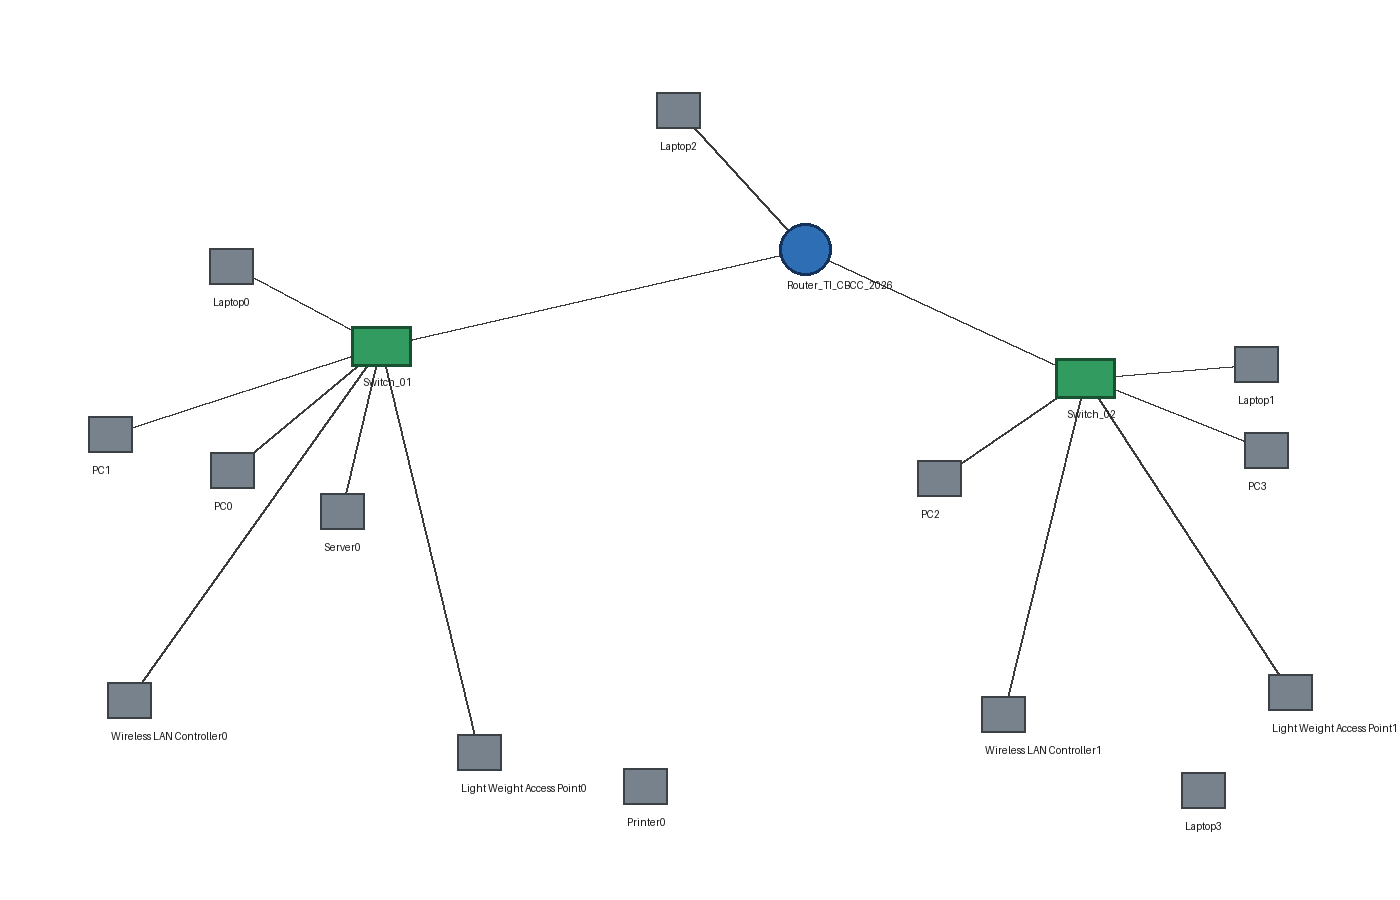
\includegraphics[width=0.88\linewidth]{pics/cenario_real.png}
    \caption{Topologia física e lógica do Cenário 03 no Cisco Packet Tracer.}
    \label{fig:topologia_real}
\end{figure}

\subsection{Interfaces de Roteamento, Gerência SVI e Endereçamento}

A Tabela~\ref{tab:ifaces} detalha a distribuição das interfaces de camada 3 ativas na topologia, com seus respectivos endereços IPv4, máscaras de sub-rede e larguras de banda atribuídas.

\begin{table}[H]
\centering
\small
\begin{tabular}{llllll}
\toprule
Roteador & Interface & IP & Prefixo & Banda & Clock/Tipo\\
\midrule
Router\_TI\_CBCC\_2026 & GigabitEthernet0/0 & 192.168.0.254 & /24 & 100 Mb/s & --\\
Router\_TI\_CBCC\_2026 & GigabitEthernet0/1 & 172.16.255.254 & /16 & 100 Mb/s & --\\
\midrule
Switch01 & Vlan1 & 192.168.0.200 & /24 & 100 Mb/s & --\\
\midrule
Switch02 & Vlan1 & 172.16.255.200 & /16 & 100 Mb/s & --\\
\bottomrule
\end{tabular}

\caption{Interfaces de Camada 3 e interfaces virtuais de comutador (SVIs).}
\label{tab:ifaces}
\end{table}

Destacam-se as Interfaces Virtuais de Comutador (\textit{Switch Virtual Interfaces} --- SVI) na VLAN 1 de gerência: o \texttt{Switch\_01} possui o endereço \texttt{192.168.0.200/24}, permitindo administração remota dentro de seu domínio local, enquanto o \texttt{Switch\_02} opera com o endereço \texttt{172.16.255.200/16}.

\subsection{Portas de Switch e Estações de Trabalho}

A ocupação física das interfaces dos comutadores \texttt{Switch\_01} e \texttt{Switch\_02} encontra-se consolidada na Tabela~\ref{tab:switchports}, enquanto os dispositivos terminais e seus pontos de terminação física estão relacionados na Tabela~\ref{tab:pcs}.

\begin{table}[H]
\centering
\small
\begin{tabular}{llll}
\toprule
Switch & Porta & Banda & Conectado a\\
\midrule
Switch\_01 & Fa0/1 & 100 Mb/s & Router\_TI\_CBCC\_2026 GigabitEthernet0/0\\
Switch\_01 & Fa0/2 & 100 Mb/s & Server0 FastEthernet0\\
Switch\_01 & Fa0/3 & 100 Mb/s & PC0 FastEthernet0\\
Switch\_01 & Fa0/4 & 100 Mb/s & PC1 FastEthernet0\\
Switch\_01 & Fa0/5 & 100 Mb/s & Light Weight Access Point0 GigabitEthernet0\\
Switch\_01 & Fa0/6 & 100 Mb/s & Wireless LAN Controller0 GigabitEthernet0\\
Switch\_01 & Fa0/7--Fa0/24, Gi0/1--Gi0/2 & 100M / 1G & Portas livres (sem conexão)\\
\midrule
Switch\_02 & Fa0/1 & 100 Mb/s & Router\_TI\_CBCC\_2026 GigabitEthernet0/1\\
Switch\_02 & Fa0/2 & 100 Mb/s & PC2 FastEthernet0\\
Switch\_02 & Fa0/3 & 100 Mb/s & PC3 FastEthernet0\\
Switch\_02 & Fa0/4 & 100 Mb/s & Light Weight Access Point1 GigabitEthernet0\\
Switch\_02 & Fa0/5 & 100 Mb/s & Wireless LAN Controller1 GigabitEthernet0\\
Switch\_02 & Fa0/6--Fa0/24, Gi0/1--Gi0/2 & 100M / 1G & Portas livres (sem conexão)\\
\bottomrule
\end{tabular}

\caption{Mapeamento posicional de portas dos comutadores Cisco Catalyst 2960.}
\label{tab:switchports}
\end{table}

\begin{table}[H]
\centering
\small
\begin{tabular}{ll}
\toprule
PC & Conectado ao Switch\\
\midrule
Laptop0 & Switch\_01 Console\\
Laptop1 & Switch\_02 Console\\
Laptop2 & Router0 Console\\
Laptop3 & --\\
PC0 & Switch\_01 Fa0/3\\
PC1 & Switch\_01 Fa0/4\\
PC2 & Switch\_02 Fa0/2\\
PC3 & Switch\_02 Fa0/3\\
Printer0 & --\\
Server0 & Switch\_01 Fa0/2\\
\bottomrule
\end{tabular}

\caption{Dispositivos finais conectados à infraestrutura.}
\label{tab:pcs}
\end{table}

\section{SERVIÇOS DE REDE, ENCAMINHAMENTO E CONFIGURAÇÕES}

\subsection{Serviço de Endereçamento Dinâmico (DHCP) e Políticas de Exclusão}

O roteador \texttt{Router\_TI\_CBCC\_2026} opera como servidor DHCP centralizado para toda a organização, provendo configuração dinâmica de pilha TCP/IP para clientes cabeados e sem fio sem a dependência de agentes \textit{DHCP Relay} intermediários, uma vez que cada uma de suas interfaces físicas atua como \textit{default gateway} diretamente inserido no respectivo segmento.

Foram configurados dois escopos (\textit{pools}) de concessão:
\begin{itemize}[leftmargin=2em]
  \item \textbf{Pool REDE192:} Associado à rede \texttt{192.168.0.0/24}, define como rota padrão o endereço \texttt{192.168.0.254} e servidor DNS \texttt{192.168.0.1}.
  \item \textbf{Pool REDE172:} Associado à rede \texttt{172.16.0.0/16}, define como rota padrão o endereço \texttt{172.16.255.254} e aponta o mesmo servidor DNS corporativo em \texttt{192.168.0.1}.
\end{itemize}

Para assegurar a integridade da rede e prevenir sobreposição ou conflitos de endereçamento IP (duplicidade de endereços), foram definidas diretivas explícitas de exclusão (\texttt{ip dhcp excluded-address}):
\begin{enumerate}[leftmargin=2em]
  \item \texttt{192.168.0.1}: Reservado para o servidor corporativo \texttt{Server0} (serviços de DNS/Web).
  \item \texttt{192.168.0.200}: Reservado para a interface SVI (\texttt{Vlan1}) do comutador \texttt{Switch\_01}.
  \item \texttt{192.168.0.254}: Reservado para a interface \texttt{GigabitEthernet0/0} do roteador (\textit{default gateway} da LAN 192).
  \item \texttt{172.16.255.200}: Reservado para a interface SVI (\texttt{Vlan1}) do comutador \texttt{Switch\_02}.
  \item \texttt{172.16.255.254}: Reservado para a interface \texttt{GigabitEthernet0/1} do roteador (\textit{default gateway} da LAN 172).
\end{enumerate}

Dessa forma, qualquer host com configuração DHCP ativada na rede (\texttt{PC0}, \texttt{PC1}, \texttt{PC2}, \texttt{PC3}, computadores portáteis e periféricos) obtém concessões seguras dentro das faixas dinâmicas disponíveis.

\subsection{Base de Informações de Roteamento (RIB)}

O roteador central interconecta diretamente as redes departamentais. Por estarem fisicamente acopladas às portas \texttt{GigabitEthernet0/0} e \texttt{GigabitEthernet0/1}, ambas as rotas figuram na tabela de roteamento como rotas diretamente conectadas (código \texttt{C}). A Tabela~\ref{tab:rib} consolida a RIB esperada do equipamento.

\begin{table}[H]
\centering
\small
\subsection*{Router\_TI\_CBCC\_2026 (Router0)}
\begin{tabular}{@{}llllp{3.6cm}@{}}\toprule Destino & Cód. & Interface de saída & Métrica & Próximo salto\\\midrule
172.16.0.0/16 & C & GigabitEthernet0/1 & -- & --\\
192.168.0.0/24 & C & GigabitEthernet0/0 & -- & --\\
\bottomrule\end{tabular}

\caption{Tabela de encaminhamento (RIB) do roteador central.}
\label{tab:rib}
\end{table}

O encaminhamento entre os pacotes originados no segmento \texttt{172.16.0.0/16} em direção aos recursos da sub-rede \texttt{192.168.0.0/24} (como as consultas enviadas ao servidor DNS \texttt{192.168.0.1}) é processado diretamente pelo roteador através de sua lógica de chaveamento de camada 3, sem a exigência de protocolos de vetor de distâncias ou estado de enlace internos na presente escala de topologia.

\subsection{Gerenciamento Out-of-Band e Infraestrutura Sem Fio}

A topologia evidencia a replicação de boas práticas de administração de infraestruturas críticas por meio de conexões seriais de console (\textit{out-of-band management}):
\begin{itemize}[leftmargin=2em]
  \item \texttt{Laptop2} conectado à porta \texttt{Console} do roteador \texttt{Router\_TI\_CBCC\_2026};
  \item \texttt{Laptop0} conectado à porta \texttt{Console} do comutador \texttt{Switch\_01};
  \item \texttt{Laptop1} conectado à porta \texttt{Console} do comutador \texttt{Switch\_02}.
\end{itemize}

Na camada de conectividade sem fio, os pontos de acesso \texttt{LAP-PT} atuam em arquitetura centralizada com os controladores \texttt{WLC-PT}. A distribuição de sinal atende a clientes sem fio como o \texttt{Laptop3} e a \texttt{Printer0}, os quais requisitam parâmetros de rede dinâmicos via DHCP e direcionam o tráfego de saída aos gateways de suas respectivas redes.

\subsection{Configurações dos Equipamentos (Running-Configs)}

A listagem a seguir reproduz fielmente as configurações essenciais extraídas dos arquivos de configuração dos dispositivos ativos presentes no arquivo de projeto:

\subsection*{Router0}
\begin{lstlisting}
hostname Router_TI_CBCC_2026
ip dhcp excluded-address 192.168.0.254
ip dhcp excluded-address 192.168.0.200
ip dhcp excluded-address 192.168.0.1
ip dhcp excluded-address 172.16.255.200
ip dhcp excluded-address 172.16.255.254
ip dhcp pool REDE192
 network 192.168.0.0 255.255.255.0
 default-router 192.168.0.254
 dns-server 192.168.0.1
ip dhcp pool REDE172
 network 172.16.0.0 255.255.0.0
 default-router 172.16.255.254
 dns-server 192.168.0.1
interface GigabitEthernet0/0
 ip address 192.168.0.254 255.255.255.0
interface GigabitEthernet0/1
 ip address 172.16.255.254 255.255.0.0
\end{lstlisting}
\subsection*{Switch\_01}
\begin{lstlisting}
hostname Switch01
interface Vlan1
 ip address 192.168.0.200 255.255.255.0
\end{lstlisting}
\subsection*{Switch\_02}
\begin{lstlisting}
hostname Switch02
interface Vlan1
 ip address 172.16.255.200 255.255.0.0
\end{lstlisting}
